\documentclass[aspectratio=169]{beamer}

\usetheme{Madrid}
\usecolortheme{default}

\usepackage[T1]{fontenc}
\usepackage{lmodern}
\usepackage{booktabs}
\usepackage{graphicx}
\usepackage{tikz}
\usetikzlibrary{arrows.meta,positioning}

\setbeamertemplate{navigation symbols}{}
\setbeamertemplate{footline}[frame number]

\title[Screen Capture Rectification]{Screen Capture Rectification and Temporal Stabilization\\for Real-world Captured-screen Videos}
\author{Rongshuo Wen \and Bihua Wen \and Ruiming Liu}
\institute{CIE6032 Final Project Proposal}
\date{June 24, 2026}

\newcommand{\imageorbox}[3]{%
  \IfFileExists{#1}{%
    \includegraphics[width=#2,height=#3,keepaspectratio]{#1}%
  }{%
    \begingroup
    \setlength{\fboxsep}{6pt}%
    \fbox{%
      \begin{minipage}[c][#3][c]{#2}
        \centering
        \scriptsize Missing image\\[2pt]
        \texttt{\detokenize{#1}}
      \end{minipage}%
    }%
    \endgroup
  }%
}

\newcommand{\smalltag}[1]{%
  \tikz[baseline=(text.base)]\node[
    fill=blue!8,
    draw=blue!30,
    rounded corners=2pt,
    inner xsep=4pt,
    inner ysep=2pt
  ] (text) {\scriptsize #1};%
}

\begin{document}

% Main talk target: 6 slides, about 3 minutes.

\begin{frame}
  \titlepage
  \vspace{-0.4cm}
  \begin{center}
    \imageorbox{assets/comparison_1s.jpg}{0.62\linewidth}{2.2cm}
  \end{center}
  \centering
  \small Before restoration, OCR, or archiving, real filmed screens first need geometric normalization.
\end{frame}

\begin{frame}{Motivation: real captured-screen videos are not pre-aligned}
  \begin{columns}[T,onlytextwidth]
    \begin{column}{0.48\textwidth}
      \imageorbox{assets/screen_corners_overlay_4s.jpg}{\linewidth}{4.3cm}
    \end{column}
    \begin{column}{0.48\textwidth}
      \begin{itemize}
        \item Many restoration datasets already assume the screen is cropped or aligned.
        \item Real phone videos include background, perspective distortion, hand shake, weak borders, glare, moire, and dynamic screen content.
        \item This project studies the missing geometric preprocessing step.
      \end{itemize}
      \vspace{0.3cm}
      \smalltag{gap: full scene input} \quad
      \smalltag{goal: stable screen coordinates}
    \end{column}
  \end{columns}
\end{frame}

\begin{frame}{Task and goal}
  \begin{columns}[T,onlytextwidth]
    \begin{column}{0.46\textwidth}
      \begin{block}{Input}
        Hand-held phone video of a computer screen.
      \end{block}
      \begin{block}{Output}
        Front-facing screen-content video with the physical aspect ratio preserved.
      \end{block}
    \end{column}
    \begin{column}{0.50\textwidth}
      \begin{itemize}
        \item Remove most non-screen background.
        \item Correct perspective distortion.
        \item Reduce frame-to-frame jitter.
        \item Preserve real screen content motion such as scrolling and video playback.
      \end{itemize}
    \end{column}
  \end{columns}
  \vfill
  \begin{center}
    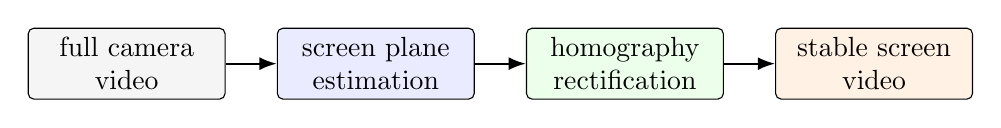
\begin{tikzpicture}[
      node distance=0.65cm,
      box/.style={draw, rounded corners=2pt, align=center, minimum height=0.75cm, minimum width=2.5cm},
      arr/.style={-{Latex[length=2.2mm]}, thick}
    ]
      \node[box, fill=gray!8] (a) {full camera\\video};
      \node[box, fill=blue!8, right=of a] (b) {screen plane\\estimation};
      \node[box, fill=green!8, right=of b] (c) {homography\\rectification};
      \node[box, fill=orange!10, right=of c] (d) {stable screen\\video};
      \draw[arr] (a) -- (b);
      \draw[arr] (b) -- (c);
      \draw[arr] (c) -- (d);
    \end{tikzpicture}
  \end{center}
\end{frame}

\begin{frame}{Core idea: estimate the physical screen plane}
  \begin{columns}[T,onlytextwidth]
    \begin{column}{0.49\textwidth}
      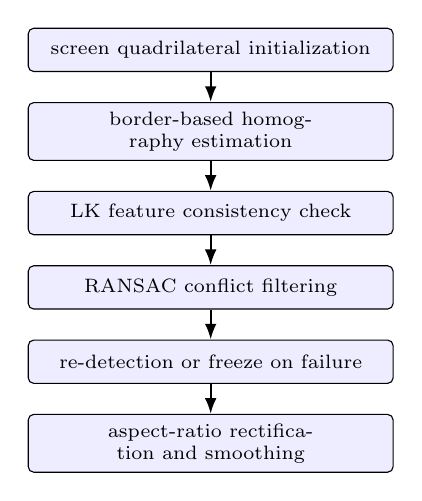
\begin{tikzpicture}[
        node distance=0.38cm,
        flowstep/.style={draw, rounded corners=2pt, align=center, minimum height=0.55cm, text width=4.4cm, font=\scriptsize},
        arr/.style={-{Latex[length=2mm]}, thick}
      ]
        \node[flowstep, fill=blue!7] (s1) {screen quadrilateral initialization};
        \node[flowstep, fill=blue!7, below=of s1] (s2) {border-based homography estimation};
        \node[flowstep, fill=blue!7, below=of s2] (s3) {LK feature consistency check};
        \node[flowstep, fill=blue!7, below=of s3] (s4) {RANSAC conflict filtering};
        \node[flowstep, fill=blue!7, below=of s4] (s5) {re-detection or freeze on failure};
        \node[flowstep, fill=blue!7, below=of s5] (s6) {aspect-ratio rectification and smoothing};
        \foreach \x/\y in {s1/s2,s2/s3,s3/s4,s4/s5,s5/s6} {
          \draw[arr] (\x) -- (\y);
        }
      \end{tikzpicture}
    \end{column}
    \begin{column}{0.49\textwidth}
      \begin{itemize}
        \item Physical borders are the main source for the screen homography.
        \item Inner LK points are used as consistency evidence, not as the main motion model.
        \item If inner motion conflicts with border motion, it is treated as screen-content motion.
        \item Corner trajectories are smoothed to suppress high-frequency jitter.
      \end{itemize}
      \vspace{0.2cm}
      \imageorbox{assets/tracking_visualization.png}{0.92\linewidth}{1.8cm}
    \end{column}
  \end{columns}
\end{frame}

\begin{frame}{Experiments and evaluation}
  \begin{columns}[T,onlytextwidth]
    \begin{column}{0.48\textwidth}
      \begin{block}{Self-collected dataset plan}
        \begin{itemize}
          \item 5 scenario classes.
          \item 10 clips per class.
          \item About 5 seconds per clip.
          \item Selected key frames manually annotated with four screen corners.
        \end{itemize}
      \end{block}
      \small Static pages, scrolling pages, in-screen video playback, PPT or weak-border pages, and glare/moire/partial-loss hard cases.
    \end{column}
    \begin{column}{0.48\textwidth}
      \begin{table}
        \scriptsize
        \begin{tabular}{@{}ll@{}}
          \toprule
          Aspect & Metrics \\
          \midrule
          Geometry & corner error, quad IoU, aspect ratio error \\
          Stability & residual translation, rotation, scale variation \\
          Signal & gradient magnitude, edge preservation index \\
          Grid/moire & 2D FFT dominant direction check \\
          \bottomrule
        \end{tabular}
      \end{table}
      \vspace{0.1cm}
      \begin{block}{Baselines}
        Frame-wise detection, content optical flow, and proposed border-guided tracking.
      \end{block}
    \end{column}
  \end{columns}
\end{frame}

\begin{frame}{Expected results and timeline}
  \begin{columns}[T,onlytextwidth]
    \begin{column}{0.45\textwidth}
      \begin{itemize}
        \item Stable front-facing videos from real captured-screen inputs.
        \item Better separation of screen-plane motion and screen-content motion.
        \item Clear failure analysis for weak borders, dynamic content, glare, and moire.
      \end{itemize}
    \end{column}
    \begin{column}{0.51\textwidth}
      \scriptsize
      \begin{tabular}{@{}ll@{}}
        \toprule
        Date & Task \\
        \midrule
        Jun. 22--24 & finalize proposal and presentation \\
        Jun. 25--26 & collect 50 self-captured clips \\
        Jun. 27--30 & organize data and annotate key frames \\
        Jul. 1--7 & run ablations and metrics \\
        Jul. 8--10 & prepare visual comparison and analysis \\
        Jul. 11--15 & finalize report, code, data, slides \\
        \bottomrule
      \end{tabular}
    \end{column}
  \end{columns}
  \vfill
  \begin{center}
    \large Deliverable: a classical geometric preprocessing pipeline for realistic filmed-screen restoration workflows.
  \end{center}
\end{frame}

\appendix

\begin{frame}{Backup for QA: why this is not a demoireing model}
  \begin{itemize}
    \item Demoireing and restoration models usually need a stable screen-coordinate input.
    \item Real usage starts with a full camera scene, not with a cropped and aligned screen.
    \item This project handles the earlier geometric stage: locate, rectify, and stabilize the screen plane.
  \end{itemize}
  \vfill
  \begin{center}
    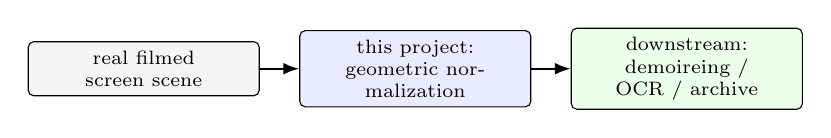
\begin{tikzpicture}[
      node distance=0.5cm,
      box/.style={draw, rounded corners=2pt, align=center, minimum height=0.65cm, text width=2.7cm, font=\scriptsize},
      arr/.style={-{Latex[length=2mm]}, thick}
    ]
      \node[box, fill=gray!8] (a) {real filmed\\screen scene};
      \node[box, fill=blue!8, right=of a] (b) {this project:\\geometric normalization};
      \node[box, fill=green!8, right=of b] (c) {downstream:\\demoireing / OCR / archive};
      \draw[arr] (a) -- (b);
      \draw[arr] (b) -- (c);
    \end{tikzpicture}
  \end{center}
\end{frame}

\begin{frame}{Backup for QA: how dynamic content is handled}
  \begin{itemize}
    \item The main homography is estimated from the physical screen boundary.
    \item Inner LK features are useful only if they agree with the screen-plane motion.
    \item RANSAC conflict filtering rejects feature motion caused by scrolling pages or in-screen playback.
    \item If confidence is low, the system re-detects the border or freezes the last valid homography and marks invalid regions.
  \end{itemize}
\end{frame}

\end{document}
